% EDITING GUIDELINES
%
% * Limit lines to no more than 100 characters.  The default should be
%   80 characters.  This leaves room for the addition of 20 new
%   characters on the same line later on.
%
%   RATIONALE: Long lines are hard to read and cause trouble when
%   viewing two versions of the file side by side (e.g., using vimdiff)
%
% * Start every sentence on a new line.
%
%   RATIONALE: This makes sentences so much easier to find using forward
%   search in emacs or vim.
%
% * Do not justify paragraphs.  Particularly, when editing an existing
%   version of the text, do not change line breaks apart from adding
%   line breaks for lines that would otherwise be too long.
%
%   RATIONALE: This makes changes from previous versions so much easier
%   to identify, particularly when using a VCS.  Adding a word and
%   justifying the paragraph may change all the lines in the paragraph,
%   making this look like a huge edit.  Without justification, the
%   diff shows only the addition of the one word.

% ------------------------------------------------------------------------------
\section{Succinct Representation of Bounded-Degree Planar Graphs}
\label{sec:graph_rep}
% ------------------------------------------------------------------------------


Our main result considers planar graphs of degree $d = \OhOf{1}$
where the degree of a graph is the maximum degree of its vertices.
Let $G$ be such a graph.
Each vertex $x$ in $G$ stores a $\bitsPerKey$-bit key
to be reported when visiting $x$.
We assume that $\bitsPerKey = \OhOf{\lg N}$, but
$\bitsPerKey$ is not necessarily related to the size of the graph.
It may take on a small constant value, e.g., the labels may be colours
chosen from a constant-size set.

Our data structure is based on a two-level partition of $G$, similar to
that used in \cite{DBLP:journals/talg/BoseCHMM12}.
More precisely, we compute an
$\regsz$-partition of $G$, for some parameter $\regsz \ge B \lg^2 N$ to be
defined later.
We refer to the subgraphs in this partition as \emph{regions}, and
denote them by $\reg[1], \reg[2], \dots, \reg[t]$.
Each region $\reg[i]$ is further
divided into smaller subgraphs, called \emph{subregions}, that form
an $\subregsz$-partition of $\reg[i]$, for some parameter
$B \le \subregsz < \regsz$.
We use $q_i$ to denote the number of subregions of $\reg[i]$, and $\subreg[i,1],
\subreg[i,2], \dots, \subreg[i,q_i]$ to denote the subregions themselves.
According to the definitions from the previous section, we classify
every vertex in a region $\reg[i]$ as a \emph{region-interior} or
\emph{region boundary vertex}, and every vertex in a subregion
$\subreg[i,j]$ as a \emph{subregion-interior} or \emph{subregion boundary
  vertex}.
Every region boundary vertex is also considered to be a
subregion boundary vertex in any subregion that contains it
(see Fig.~\ref{fig:partitioned_graph} for an illustration).
Note that if a vertex is a region boundary vertex of one region, it is a region
boundary vertex for all regions that contain it.
The same is true for subregion boundary vertices.
Thus, we can refer to a vertex as a region or subregion boundary or interior
vertex without reference to a specific region or subregion.

% ------------------------------------------------------------------------------
\begin{figure}[t]
  \centering
  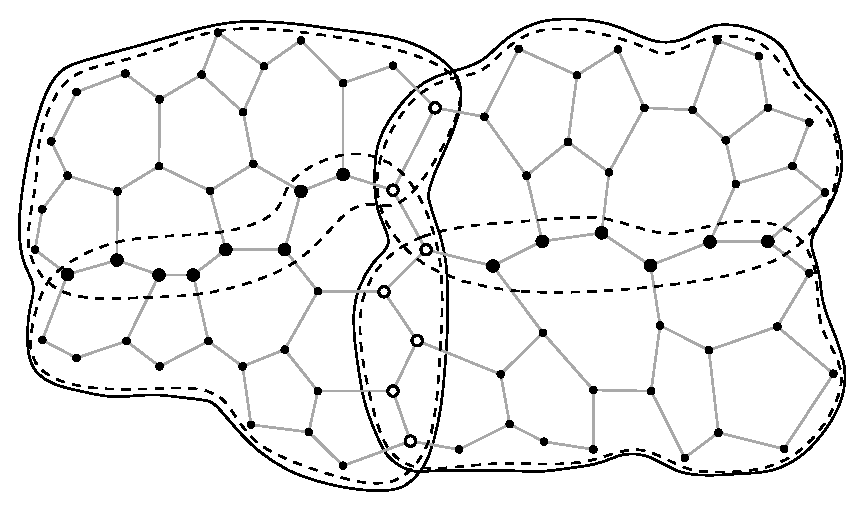
\includegraphics[width=0.6\textwidth]{Fig1}
  \caption[Recursively-partitioned graph]{A graph $G$ partitioned into two 
	regions (delineated by solid lines), which are further partitioned into two 
	subregions each (delineated by dashed lines).
    Region boundary vertices are shown as large hollow disks while subregion 
	boundary vertices interior to their regions are shown as large solid disks.
    Vertices interior to their subregions are shown as small solid disks.}
  \label{fig:partitioned_graph}
\end{figure}
% ------------------------------------------------------------------------------

In our data structure, all subregions are stored explicitly while
regions are represented implicitly as unions of their subregions.
In addition, we store the \emph{$\alpha$-neighbourhoods} of all (region
and subregion) boundary vertices.
These neighbourhoods are defined
as follows~\cite{DBLP:conf/soda/AgarwalAMVV98}.
For a vertex $x$, consider a breadth-first search in $G$ starting at $x$.
Then the $\alpha$-neighbourhood $\nb[\alpha]{x}$ of $x$ is the subgraph of $G$
induced by the first $\alpha$ vertices visited by the search.
For a region boundary vertex, we store its entire $\alpha$-neighbourhood.
For a subregion boundary vertex interior to a region $\reg[i]$, we store
only those vertices of its $\alpha$-neighbourhood that belong to
$\reg[i]$.
A vertex $y \in \nb[\alpha]{x}$ is an \emph{interior vertex} of
$N_\alpha(x)$ if all its neighbours belong to $\nb[\alpha]{x}$;
otherwise $y$ is \emph{terminal}
(see Fig.~\ref{fig:alpha_neighbourhoods} for an illustration of the
definitions pertaining to $\alpha$-neighbourhoods).

% ------------------------------------------------------------------------------
\begin{figure}[t]
  \centering
  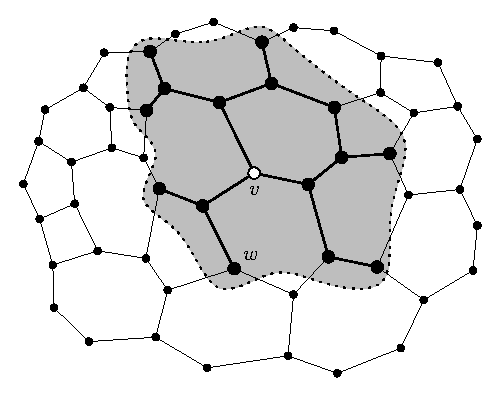
\includegraphics{Fig2}
  \caption[$\alpha$-neighbourhood of a boundary vertex]{The 
	$\alpha$-neighbourhood $\nb[\alpha]{v}$ of a vertex $v$,
    for $\alpha = 16$.
    Vertex $v$ is interior to $\nb[\alpha]{v}$ while vertex $w$ is terminal.}
  \label{fig:alpha_neighbourhoods}
\end{figure}
% ------------------------------------------------------------------------------

We refer to subregions and $\alpha$-neighbourhoods---that is, to the
subgraphs of $G$ we store explicitly---as \emph{components} of $G$.
We store each component succinctly so as to allow for the efficient
traversal of edges in the component.
The traversal of a path in $G$ must be able to visit different components.
In order to facilitate this, we assign a unique \emph{graph label} to each vertex of $G$
and provide mechanisms to (1) identify a component containing a vertex $x$ and
locate $x$ in that component, given its graph label, and (2) determine
the graph label of any vertex in a given component.

The rest of this section is organized as follows.
In Section~\ref{sec:graph_labelling}, we define a number of labels
assigned to the vertices of $G$, including the graph labels just
mentioned, and provide $\ohOf{N}$-bit data structures that allow us to
convert any such label into any other label using $\OhOf{1}$ I/Os.
In Section~\ref{sec:datastructs}, we discuss the succinct
representations we use to store subregions and
$\alpha$-neighbourhoods.
In Section~\ref{sec:navigation},
we discuss how to traverse paths I/O efficiently using this
representation.
In Section \ref{sec:alt_block_scheme}, we describe an 
alternative scheme
for blocking planar graphs that can improve I/O efficiency in 
some instances.

% ------------------------------------------------------------------------------
\subsection{Graph Labeling}
% ------------------------------------------------------------------------------

\label{sec:graph_labelling}

In this section, we describe the labeling scheme that underlies our
data structure.
Our scheme is based on the one used in
Bose~\etal~\cite{DBLP:journals/talg/BoseCHMM12}.
It assigns three labels to each vertex.
As already mentioned, the \emph{graph label} $\glbl{x}$ identifies each vertex
$x \in G$ uniquely.
The \emph{region label} $\reglbl[i]{x}$ of a vertex $x$ in a region $\reg[i]$
identifies $x$ uniquely among the vertices in $\reg[i]$, and the
\emph{subregion label} $\subreglbl[i,j]{x}$ of a vertex $x$ in a subregion
$\subreg[i,j]$ identifies $x$ uniquely
among the vertices in $\subreg[i,j]$.
(Note that a region boundary vertex appears in more than one region and,
thus, receives one region label per region that contains it.
Similarly, every region or subregion boundary vertex receives multiple
subregion labels.)

A standard data structure would identify vertices by their graph labels and
store these labels for every vertex.
Since there are $N$ vertices, every graph label must use at least
$\lg N$ bits, and such a representation uses at least $N \lg N$ bits of space.
In our structure, we store graph labels for only a small subset of the vertices, 
region labels for yet another subset of the vertices, and subregion labels for 
a third subset. 
Many vertices in the graph have no label explicitly stored.
Since regions and subregions are small, and region and subregion labels have to
be unique only within a region or subregion, they can be stored using
less than $\lg N$ bits each.
Next we define these labels.

In the data structure described in the next section, the vertices of
each subregion $\subreg[i,j]$ are stored in a particular order $\perm[i,j]$.
We use the position of a vertex $x$ in $\perm[i,j]$ as its
subregion label $\subreglbl[i,j]{x}$ for subregion~$\subreg[i,j]$.

For a region $\reg[i]$ and a vertex $x \in \reg[i]$, we say an occurrence of
$x$ in a subregion $\subreg[i,j]$ \emph{defines} $x$ if there is no
subregion $\subreg[i,h]$ with $h < j$ that contains~$x$; otherwise the
occurrence is a \emph{duplicate}.
If the occurrence of $x$ in a subregion $\subreg[i,j]$ defines $x$, we also call
$\reg[i,j]$ the \emph{defining subregion} of $x$.
Clearly, all occurrences of subregion interior vertices are
defining.
We order \footnote{This ordering, as with the ordering used for assigning 
graph labels, is employed strictly for labeling purposes. It does not imply
any arrangement of vertices within the structures used to represent the graph.}
the vertices of $\reg[i]$ so that all subregion boundary vertices
precede all subregion-interior vertices, and the vertices in each of these two
groups are sorted primarily by their defining subregions and secondarily by
their subregion labels within these subregions.
The region labels of the vertices in $\reg[i]$ are now obtained by numbering the
vertices in this order.


Graph labels are defined analogously to region labels.
Again, we say an occurrence of a vertex $x$ in a region $\reg[i]$ defines
$x$ if $x \not\in \reg[h]$, for all $h < i$.
We then order the vertices of $G$ so that the region boundary vertices precede
the region-interior vertices, and the vertices in each of these two groups are
sorted primarily by their defining regions and secondarily by their region
labels inside their defining regions.
The graph labels of the vertices in $G$ are
then obtained by numbering the vertices in order.

Observe that this labeling scheme ensures that all vertices interior
to a region $\reg[i]$ receive consecutive graph labels, and all vertices
interior to a subregion $\subreg[i,j]$ receive consecutive graph and
region labels.
Our data structure for representing the graph $G$ will make use of
the following result, which extends a result from \cite{DBLP:journals/talg/BoseCHMM12}.
In particular, parts~\ref{item:subregion-to-region}
and~\ref{item:region-to-graph} were proved in \cite{DBLP:journals/talg/BoseCHMM12} for a slightly
different vertex labeling than we use here while
parts~\ref{item:graph-to-region} and~\ref{item:region-to-subregion} are new.
For completeness, we prove all parts of the lemma here.

% ------------------------------------------------------------------------------
\begin{lemma}
  \label{lem:label_ops}
  There is a data structure of $\ohOf{N}$ bits that allows the following
  conversion between vertex labels of $G$ to be performed using
  $\OhOf{1}$ I/Os.
  \begin{enumerate}[label={(\alph{*})},noitemsep]
  \item Given the graph label $\glbl{x}$ of a vertex $x$, compute the defining
    region $\reg[i]$ of $x$ and the region label $\reglbl[i]{x}$ of $x$ in
    $\reg[i]$.\label{item:graph-to-region}
  \item Given the region label $\reglbl[i]{x}$ of a vertex $x$ in a region
    $\reg[i]$, compute the defining subregion $\subreg[i,j]$ of $x$ and the
    subregion label $\subreglbl[i,j]{x}$ of $x$ in
    $\subreg[i,j]$.\label{item:region-to-subregion}
  \item Given the subregion label of a vertex $x$ in a subregion
    $\subreg[i,j]$ of $\reg[i]$, compute the region label $\reglbl[i]{x}$
    of $x$ in $\reg[i]$.\label{item:subregion-to-region}
  \item Given the region label of a vertex $x$ in a region $\reg[i]$,
    compute the graph label $\glbl{x}$ of $x$.\label{item:region-to-graph}
  \end{enumerate}
\end{lemma}
% ------------------------------------------------------------------------------

\begin{proof}
  We construct separate $\ohOf{N}$-bit data structures in order to accomplish parts
  \ref{item:region-to-subregion} and~\ref{item:subregion-to-region}, and to
  accomplish parts \ref{item:graph-to-region} and~\ref{item:region-to-graph}.
  Since these data structures are very similar, we discuss those for
  parts \ref{item:region-to-subregion} and~\ref{item:subregion-to-region} in detail,
  and only provide a space analysis for the second structure.
  We use $\numv[i]$ to denote the number of vertices in region $\reg[i]$,
  $\numv[i,j]$ to denote the number of vertices in subregion $\subreg[i,j]$,
  $\dnumv[i] := \sum_{j=1}^{q_i} \numv[i,j]$ to denote the total number of
  vertices in all subregions of~$\reg[i]$, where $q_i$ is the number of
  subregions of region $\reg[i]$, and $\dnumv := \sum_{i=1}^t \dnumv[i]$ to
  denote the total number of vertices in all subregions.

  Our data structure for converting between region and subregion labels consists
  of a number of vectors.
  We introduce them as required for the operations we discuss.
  Most of these vectors are bit vectors representing a vector $\vvec$
  of the vertices in all subregions of $G$.
  We define this vector first.
  $\vvec$ is the concatenation of $t$ subvectors $\vvec[1], \vvec[2],
  \dots, \vvec[t]$ storing the vertices in the regions of $G$.
  Each such vector $\vvec[i]$ is itself the concatenation of
  subvectors $\vvec[i,1], \vvec[i,2], \dots, \vvec[i,q_i]$ representing
  the subregions of $\reg[i]$.
  Each such vector $\vvec[i,j]$ stores the vertices in $\subreg[i,j]$
  sorted by their subregion labels.
  Note that our data structure does not store $\vvec$.
  We only introduce it here as a reference for discussing the vectors our
  data structure does store.
  Throughout this proof, when we define a bit vector, we store it using
  the second part of Lemma~\ref{lem:rank_select} to support constant-I/O
  accesses to its elements, as well as constant-I/O $\rankopsym$ and $\selopsym$
  operations.

\begin{table*}[ht]
	\centering
		\begin{tabular}{ l | l}
			Operator & Description \\ \hline
			$\rankop[x]{S, i}$ & Returns the number of $x$'s in bit-vector $S$ up to
				position $S[1..i]$, where $x \in \{0,1\}$.\\
			$\selop[x]{S, r}$ & Returns the $r$\textsuperscript{th} $x$ in bit-vector $S$
				where $x \in \{0,1\}$.\\
			$\regpos{i}$ & Returns the first element of region $\reg[i]$ in $\vvec$. \\
			$\subregpos{i,j}$ & Returns the first element of sub-region $\subreg[i,j]$
				in $\vvec$. \\
			$\possubreg{i,p}$ & Returns the sub-region index $j$ from $\vvec$ where
				$p \in \reg[i]$. \\
			$\bdcount{i}$ & Calculates in $\vvec$ the number of sub-region boundary vertices
				in $\reg[i]$. \\ \hline
		\end{tabular}
	\caption{Summary of bit-vector operations used in this section. }
	\label{tab:succ_operators}
\end{table*}

  % ------------------------------------------------------------------
  \paragraph{Locating subvectors.}
  % ------------------------------------------------------------------

  The first two vectors that our data structure stores are bit vectors
  $\fstofreg$ and $\fstofsubreg$ that
  allow us to identify, for a region $\reg[i]$, the index of the first
  element of $\vvec[i]$ in $\vvec$ and, for a subregion $\subreg[i,j]$,
  the index of the first element of $\vvec[i,j]$ in $\vvec$.
  Both vectors have length $\dnumv = \size{\vvec}$.
  The $k$th bit in $\fstofreg$ is $1$ if and only if $\vvec[][k]$ is the
  first element of $\vvec[i]$, for some region $\reg[i]$,
  and the $k$th bit of $\fstofsubreg$ is $1$
  if and only if $\vvec[][k]$ is the first element of $\vvec[i,j]$, for some
  subregion $\subreg[i,j]$.
  Using these two bit vectors, we can implement the following three operations
  using $\OhOf{1}$ I/Os.
  \begin{itemize}
  \item $\regpos{i}$ returns the index of the first element of $\vvec[i]$
    in $\vvec$ and is implemented as $\regpos{i} := \selop[1]{\fstofreg,i}$.
  \item $\subregpos{i,j}$ returns the index of the first element of $\vvec[i,j]$
    in $\vvec$ and is implemented as
    $\subregpos{i,j} := \selop[1]{\fstofsubreg,\rankop[1]{\fstofsubreg,\regpos{i}-1}+j}$.
  \item $\possubreg{i,p}$ returns the index $j$ of the subregion $\subreg[i,j]$
    of $\reg[i]$ such that $\vvec[][p]$ is an element of  $\vvec[i,j]$,
    provided $\vvec[][p]$ is an element of $\vvec[i]$.
    This operation can be implemented as
    $\possubreg{i,p} := \rankop[1]{\fstofsubreg,p} - \rankop[1]{\fstofsubreg,
      \regpos{i} - 1}$.
  \end{itemize}

  % ------------------------------------------------------------------
  \paragraph{Identifying subregion boundary vertices.}
  % ------------------------------------------------------------------

  The next two vectors we store, $\idxvec$ and $\bdvec$, help us decide whether
  a vertex is a subregion boundary vertex based only on its region or subregion
  label.
  This is useful because the conversion between region and subregion
  labels is done differently for subregion boundary and subregion-interior
  vertices.
  Vector $\idxvec$ is the concatenation of $t$ bit vectors
  $\idxvec[1], \idxvec[2], \dots, \idxvec[t+1]$.
  For $1 \le i \le t$, the subvector $\idxvec[i]$ has length equal to the
  number of subregion boundary vertices in $\reg[i]$.
  Its first bit is $1$, all other bits are $0$.
  The last subvector $\idxvec[t+1]$ stores a single $1$ bit.
  Vector $\bdvec$ is a bit vector of length $n'$.
  $\bdvec[][k] = 1$ if and only if $\vvec[][k]$ is a subregion boundary
  vertex.

  Now observe that a vertex $x$ with region label $\reglbl[i]{x}$ in region
  $\reg[i]$ is a subregion boundary vertex if and only if
  $\reglbl[i]{x}$ is no greater than the number of subregion boundary vertices
  in $\reg[i]$ because, in the ordering used to define
  the region labels of the vertices in $\reg[i]$, all subregion boundary
  vertices precede all subregion-interior vertices.
  In order to test this condition, we need to compute the number of subregion
  boundary vertices in $\reg[i]$, which we can do using $\OhOf{1}$ I/Os
  as $\bdcount{i} := \selop[1]{\idxvec,i+1} - \selop[1]{\idxvec,i}$.
 
  For a vertex $x$ with subregion label $\subreglbl[i,j]{x}$ in subregion
  $\subreg[i,j]$, observe that the subvector $\vvec[i,j]$ of $\vvec$
  stores the vertices of $\subreg[i,j]$ sorted by their subregion labels.
  Thus, $x$ appears at position $\subreglbl[i,j]{x}$ in $\vvec[i,j]$,
  which is position $k := \subregpos{i,j} + \subreglbl[i,j]{x} - 1$ in $\vvec$.
  The corresponding bit $\bdvec[][k]$ in $\bdvec$ is $1$ if and only if
  $x$ is a subregion boundary vertex.
  Thus, testing whether $x$ is a subregion boundary vertex requires calculating
  $\subregpos{i,j}$, which takes $\OhOf{1}$ I/Os followed by a single lookup
  in the bit vector $\bdvec$.

  % ------------------------------------------------------------------
  \paragraph{Subregion-interior vertices.}
  % ------------------------------------------------------------------

  For the set of subregion-interior vertices, the vectors we have already
  defined suffice to convert between region
  and subregion labels.

  Given a subregion-interior vertex $x$ in $\reg[i]$ and its region label
  $\reglbl[i]{x}$ in $\reg[i]$, observe that the subregion-interior vertices in
  $\reg[i]$ appear in $\vvec[i]$ sorted by their region labels, and
  that these are exactly the vertices in $\vvec[i]$ whose corresponding
  bits in $\bdvec$ are $0$.
  Thus, since subregion-interior vertices have greater region labels than
  subregion boundary vertices, we can find the position $k$ of the only
  occurrence of $x$ in $\vvec$ as
  $k := \selop[0]{\bdvec, \rankop[0]{\bdvec, \regpos{i} - 1} + \reglbl[i]{x} 
  - \bdcount{i}}$, which takes $\OhOf{1}$ I/Os to compute.
  Vertex $x$ belongs to the subregion $\subreg[i,j]$ such that
  $\vvec[][k]$ belongs to $\vvec[i,j]$.
  The index $j$ of this subregion is easily computed using $\OhOf{1}$ I/Os, as
  $j := \rankop[1]{\fstofsubreg,k} - \rankop[1]{\fstofsubreg,\regpos{i}-1}$.
  Since vertices in $\vvec[i,j]$ are sorted by their subregion labels in
  $\subreg[i,j]$, the subregion label of $x$ is the index of $\vvec[][k]$
  in $\vvec[i,j]$, which can be computed using $\OhOf{1}$ I/Os as
  $\subreglbl[i,j]{x} := k - \subregpos{i,j} + 1$.

  To compute the region label in $\reg[i]$ for a subregion-interior
  vertex $x$ in $\subreg[i,j]$, we perform this conversion in the reverse
  direction.
  Firstly, we find the position $k$ of $x$ in $\vvec$ as
  $k := \subregpos{i,j} + \subreglbl[i,j]{x} - 1$.
  Secondly, we compute the region label of $x$ in $\reg[i]$ as
  $\reglbl[i]{x} := \rankop[0]{\bdvec,k} - \rankop[0]{\bdvec,\regpos{i}-1} + \bdcount{i}$,
  which is correct by the argument from the previous paragraph.
  Thus, the conversion from subregion labels to region labels also takes
  $\OhOf{1}$ I/Os.

  % ------------------------------------------------------------------
  \paragraph{Subregion boundary vertices.}
  % ------------------------------------------------------------------

  For subregion boundary vertices in $\reg[i]$, the vectors we have defined so
  far cannot be used to convert between region and subregion labels, mainly
  because these vertices by definition appear more than once in $\vvec[i]$.
  On the other hand, there are only a few such vertices, which allows us to
  store their region and subregion labels explicitly.
  In particular, we store two vectors $\regvec$ and~$\subregvec$.
  Vector $\regvec$ is the concatenation of subvectors $\regvec[1], \regvec[2],
  \dots, \regvec[t]$, one per region $\reg[i]$ of $G$.
  The length of $\regvec[i]$ is the number of subregion boundary vertices
  in $\reg[i]$, and $\regvec[i][k]$ is the pair $(j,k')$ such that the
  subregion $\subreg[i,j]$ is the defining subregion of the vertex $x$
  with region label $k$, and $k'$ is $x$'s subregion label in $\subreg[i,j]$.
  We represent the index $j$ using $\lg \regsz$ bits, and the subregion
  label $k'$ using $\lg \subregsz$ bits.
  The length of vector $\subregvec$ equals the number of $1$s in vector
  $\bdvec$.
  $\subregvec[][k]$ is the region label of the vertex in $\vvec$ corresponding
  to the $k$th $1$ in $\bdvec$.
  We store each such region label in $\subregvec$ using $\lg \regsz$ bits.

  Now consider a subregion boundary vertex $x$ with region label
  $\reglbl[i]{x}$ in $\reg[i]$.
  The index of the entry in $\regvec$ storing the index of the defining
  subregion of $x$ and $x$'s subregion label in this subregion is 
  $k := \selop[1]{\idxvec,i} + \reglbl[i]{x} - 1$, which takes
  $\OhOf{1}$ I/Os to compute.
  Another I/O suffices to retrieve $\regvec[][k]$.

  Given a subregion boundary vertex $x$ with subregion label
  $\subreglbl[i,j]{x}$ in subregion $\subreg[i,j]$, the index of $x$ in
  $\vvec$ is $k := \subregpos{i,j} + \subreglbl[i,j]{x} - 1$.
  The corresponding bit $\bdvec[][k]$ in $\bdvec$ is $1$, and the
  region label of $x$ can be retrieved from
  $\subregvec[][\rankop[1]{\bdvec,k}]$, which takes $\OhOf{1}$ I/Os.

  % ------------------------------------------------------------------
  \paragraph{Space bound.}
  % ------------------------------------------------------------------

  The vectors $\fstofreg$ and $\fstofsubreg$ have length
  $n' = N + \OhOf{N / \sqrt{\subregsz}} = \OhOf{N}$ because their length
  equals that of $\vvec$; only subregion boundary vertices appear more
  than once in $\vvec$, and the total number of occurrences of subregion
  boundary vertices in $\vvec$ is $\OhOf{N / \sqrt{\subregsz}}$ by
  Lemma~\ref{lem:fred_graph_sep}.
  Every $1$-bit in such a vector corresponds to the start of a region
  or subregion.
  Thus, both vectors contain $\OhOf{N / \subregsz} = \ohOf{N}$ $1$s.
  By Lemma~\ref{lem:rank_select}(b), this implies that both vectors can
  be represented using $\ohOf{N}$ bits.

  The vector $\idxvec$ has length $\OhOf{N / \sqrt{\subregsz}} = \ohOf{N}$
  because every bit in $\idxvec$ corresponds to a unique subregion boundary
  vertex.
  Thus, by Lemma~\ref{lem:rank_select}(a), we can store $\idxvec$ using
  $\ohOf{N}$ bits.

  The vector $\bdvec$ has length $n' = \OhOf{N}$ and contains
  $\OhOf{N / \sqrt{\subregsz}}$ $1$s, one per occurrence of a subregion boundary
  vertex in a subregion.
  Hence, by Lemma~\ref{lem:rank_select}(b), we can store $\bdvec$ using
  $\ohOf{N}$ bits.

  Finally, the number of entries in vectors $\regvec$ and $\subregvec$ is
  bounded by the number of occurrences of subregion boundary vertices in
  subregions, which is $\OhOf{N / \sqrt{\subregsz}}$.
  Each entry in such a vector is represented using
  $\OhOf{\lg \regsz} = \OhOf{\lg\subregsz + \lg \lg N}$ bits.
  Thus, the total space used by these two vectors is
  $\OhOf{(N / \sqrt{\subregsz})(\lg \subregsz + \lg \lg N)}$,
  which is $\ohOf{N}$ because $\subregsz = B = \OmegaOf{\lg N}$.
  To summarize, the vectors we use to convert between region and subregion
  labels use $\ohOf{N}$ space and allow us to convert between these labels
  using $\OhOf{1}$ I/Os.
  This proves parts (b) and (c) of the lemma.

  % ------------------------------------------------------------------
  \paragraph{Conversion between region and graph labels.}
  % ------------------------------------------------------------------

  The data structure for conversion between region and graph labels is
  identical, with the following modifications.
  \begin{itemize}
  \item The vector $\vvec$ is the concatenation of $t$ subvectors
    $\vvec[1], \vvec[2], \dots, \vvec[t]$.
    Vector $\vvec[i]$ stores the vertices in region $\reg[i]$ sorted
    by their region labels.
  \item The $k$th bit in $\bdvec$ is one if and only if the vertex
    $\vvec[k]$ is a region boundary vertex.
  \item There is no need for vectors $\fstofsubreg$ and $\idxvec$.
    Instead, we store a single $(\lg N)$-bit integer counting the number
    of region boundary vertices of $G$.
  \item The entries in $\regvec$ are pairs of indices of defining
    regions and region labels in these regions, and the entries in
    $\subregvec$ are graph labels.
  \end{itemize}
  Using these modified vectors, the conversion between graph and region labels
  can be accomplished using straightforward modifications of the procedures
  described in this proof.

  Vectors $\fstofreg$ and $\bdvec$ have length
  $N + \OhOf{N / \sqrt{\regsz}} = \OhOf{N}$ and contain $\OhOf{N / \regsz}$ and
  $\OhOf{N / \sqrt{\regsz}}$ $1$s, respectively, which are both $\ohOf{N}$.
  Hence, by Lemma~\ref{lem:rank_select}(b), they can both be stored using
  $\ohOf{N}$ bits.
  The number of region boundary vertices is stored using $\lg N = \ohOf{N}$
  bits.
  Each entry in vectors $\regvec$ and $\subregvec$ uses $\OhOf{\lg N}$ bits
  of space, and the number of these entries is $\OhOf{N / \sqrt{\regsz}}$.
  Hence, the total size of these vectors is $\OhOf{(N / \sqrt{\regsz}) \lg N}$,
  which is $\ohOf{N}$ because $\regsz \ge B \lg^2 N = \OmegaOf{\lg^3 N}$.
  This proves parts (a) and (d) of the lemma.
\end{proof}

% ------------------------------------------------------------------------------
\subsection{Data Structures}\label{sec:datastructs}
% ------------------------------------------------------------------------------

Our representation of $G$ consists of three parts: (1) succinct
representations of the subregions, packed into an array $\ds$, (2)
succinct representations of the $\alpha$-neighbourhoods of boundary
vertices, packed into two array $\regnbvec$ and $\subregnbvec$, and (3) two
vectors $\regminvec$ and $\subregminvec$ recording the minimum graph labels of
the interior vertices in each region or subregion.
Throughout this section, we use total orders $\reglt$ and $\subreglt$ of the
regions and subregions of~$G$, respectively.
For two regions $\reg[i]$ and $\reg[j]$, we define $\reg[i] \reglt \reg[j]$ if
$i < j$.
For two subregions $\subreg[i,j]$ and $\subreg[i',j']$, we define
$\subreg[i,j] \subreglt \subreg[i',j']$ if $i < i'$ or $i = i'$ and $j < j'$.

% ------------------------------------------------------------------------------
\paragraph{Minimum graph labels.}
% ------------------------------------------------------------------------------

The first part of our data structure consists of two arrays $\regminvec$ and
$\subregminvec$.
The $k$\textsuperscript{th} position of $\regminvec$ stores the minimum graph
label of the interior vertices in region $\reg[k]$.
The $k$\textsuperscript{th} position in $\subregminvec$ stores the minimum graph label of the
interior vertices in the subregion $\subreg[i,j]$ at position $k$ in the
sequence of subregions defined by $\subreglt$.

% ------------------------------------------------------------------------------
\paragraph{Succinct encoding of subregions.}
% ------------------------------------------------------------------------------

We represent each subregion $\subreg[i,j]$ using four data structures:
\begin{enumerate}
\item Its number of vertices $\numv[i,j]$ stored in $\lg N$
  bits.\footnote{$\lg \subregsz$ bits would suffice; however it simplifies the
    analysis to use $\lg N$ bits.}
\item The graph structure of $\subreg[i,j]$ encoded succintly as
	$\graphrep[i,j]$, using the encoding of 
	\cite{DBLP:journals/siamcomp/ChiangLL05}.
  This encoding involves a permutation $\perm[i,j]$ of
  the vertices in $\subreg[i,j]$.
\item A bit vector $\bdvec[i,j]$ of length $\size{\subreg[i,j]}$ with
  $\bdvec[i,j][i] = 1$ if and only if the corresponding vertex in $\perm[i,j]$
  is a  (region or subregion) boundary vertex.
\item An array $\keyvec[i,j]$ of length $\size{\subreg[i,j]}$ that stores the
  $\bitsPerKey$-bit key for each vertex.
  These labels are stored according to the permutation $\perm[i,j]$.
\end{enumerate}
The representation of $\subreg[i,j]$ is the concatenation of $\numv[i,j]$,
$\graphrep[i,j]$, $\bdvec[i,j]$, and $\keyvec[i,j]$.

Let $\succblksize$ be the maximum integer such that a subregion with $\succblksize$
vertices can be encoded in this manner. 
We choose the parameters of our two-level partition as $\regsz := \succblksize \log^3
N$ and $\subregsz := \succblksize$.
This ensures that every subregion fits in a disk block.
However, a given subregion may be much smaller, and storing
each subregion in its own disk block may be wasteful.
Instead, we pack the representations of all subregions into an array $\ds$,
without gaps, using a construction proposed 
in~\cite{DBLP:journals/algorithmica/DillabaughHM12} as follows.
The subregion representations in $\ds$ are ordered according to $\subreglt$
and the array $\ds$ is stored in consecutive disk blocks; the first
$\lg N$ bits of each block are reserved for a \emph{block offset}
value.
Note that the representation of each region $\subreg[i,j]$ is
distributed over at most two consecutive blocks in $\ds$.
If $\subreg[i,j]$ is distributed over two blocks $B_1$ and $B_2$,
the block offset of the second block, $B_2$, records the number of bits
of $\subreg[i,j]$ stored in $B_2$.
Any other block stores a block offset of~$0$.
In other words, the block offset of each block stores the starting
position of the first region $\subreg[i,j]$ in this block that is not
stored partially in the previous block.
Since we use $\lg N$ bits per block to store the block offset, each subregion
of size $\succblksize$ must be stored in at most $B \wsize - \lg N$ bits.
This representation of $\ds$ is illustrated in Figure~\ref{fig:block-packing}.
 

% ------------------------------------------------------------------------------
\begin{figure}[t]
  \centering
  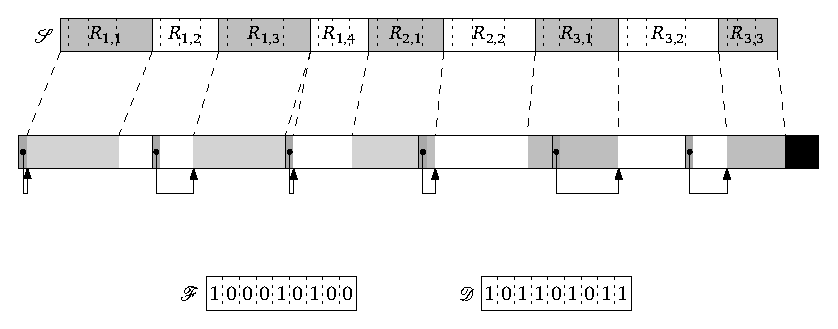
\includegraphics{Fig3}
  \caption[Packing graph blocks in memory]{Arrays $\ds$, $\fst$, and $\diff$ 
	and the packing of $\ds$ into blocks.
    The dark portion at the beginning of each block stores the block offset.
    The black portion of the last block is unused.}
  \label{fig:block-packing}
\end{figure}
% ------------------------------------------------------------------------------

In order to facilitate the efficient lookup of subregions in $\ds$, we augment
it with two bit vectors $\fst$ and $\diff$, each represented to support
constant-time $\rankop$ and $\selop$ queries (see Lemma~\ref{lem:rank_select}).
If $Q$ is the total number of subregions in~$G$, each of the two vectors has
length $Q$.
Their entries are defined as follows:
\begin{enumerate}
\item $\fst[k] = 1$ if and only if the $k$th subregion $\subreg[i,j]$
  is the first subregion in $\reg[i]$; that is, if $j = 1$.
\item $\diff[k] = 1$ if and only if the $k$th subregion starts in
  a different block from the $(k-1)$st subregion, that is, if
  the first bits of these two regions belong to different blocks in
  $\ds$.
\end{enumerate}

% ------------------------------------------------------------------------------
\paragraph{\boldmath Succinct encoding of $\alpha$-neighbourhoods.}
% ------------------------------------------------------------------------------

The third piece of our data structure consists of succinct encodings
of the $\alpha$-neighbourhoods of (region and subregion) boundary
vertices, for $\alpha = (\succblksize)^{1/3}$.
Recall that the $\alpha$-neighbourhood of a subregion boundary vertex interior
to its region includes only vertices inside this region.
Each $\alpha$-neighbourhood $\nb[\alpha]{x}$ is represented using the
following structures:
\begin{enumerate}
\item A succinct encoding $\graphrep[x]$ of the graph structure of
  $\nb[\alpha]{x}$.
  This encoding involves a permutation $\perm[x]$ of the vertices in
  $\nb[\alpha]{x}$.
\item A bit vector $\term[x]$ of length $\size{\nb[\alpha]{x}}$ for which
  $\term[x][k] = 1$ if and only if the $k$th vertex in $\perm{x}$ is a terminal
  vertex of $\nb[\alpha]{x}$.
\item A $(\lg \alpha)$-bit integer $\pos[x]$ that records the position of
  $x$ in $\perm[x]$.
\item An array $\keyvec[x]$ of length $\size{\nb[\alpha]{x}}$ that stores the
  key associated with each vertex in $\nb[\alpha]{x}$.
  These keys are stored according to the permutation $\perm[x]$.
\item An array $\lblvec[x]$ of length $\size{\nb[\alpha]{x}}$ that stores
  labels of the vertices in $\nb[\alpha]{x}$.
  The specific labels stored in $\lblvec[x]$ depend on whether $x$ is a region
  boundary vertex or a subregion boundary vertex interior to a region.
  \begin{itemize}
  \item If $x$ is a region boundary vertex, $\lblvec[x][k]$ is the graph
    label of the $k$th vertex in $\perm[x]$.
    Each such graph label is stored using $\lg n$ bits.
  \item If $x$ is a subregion boundary vertex interior to a region
    $\reg[i]$, the label stored in $\lblvec[x][k]$ depends on the type of the
    $k$\textsuperscript{th} vertex $y$ in $\perm[x]$.
    If $y$ is an interior vertex of $\nb[\alpha]{x}$---that is,
    $\term[x][k] = 0$---then $\lblvec[x][k]$ is the difference between the graph
    label of $y$ and the minimum graph label of the interior vertices in
    $\reg[i]$,  which is stored in $\regminvec$.
    We call this the \emph{region offset} of $y$.
    If $y$ is a terminal vertex of $\nb[\alpha]{x}$---that is,
    $\term[x][k] = 1$---then $\lblvec[x][k]$ is the region label of $y$.
    We note that each of these two types of labels can be stored using
    $\lg \regsz$ bits.
    For region labels this is obvious, as each region has at most $\regsz$
    vertices.
    For region offsets, we observe that every interior vertex of
    $\nb[\alpha]{x}$ must also be interior to $\reg[i]$ because every
    boundary vertex of $\reg[i]$ has at least one neighbour outside of
    $\reg[i]$ and, hence, must be terminal for $\nb[\alpha]{x}$ (if it is
    contained in $\nb[\alpha]{x}$) because $\nb[\alpha]{x}$ contains only
    vertices in $\reg[i]$.
    The bound on the number of bits required to store region offsets now
    follows because $\reg[i]$ has at most $\regsz$ vertices, and all interior
    vertices of $\reg[i]$ receive consecutive graph labels.
  \end{itemize}
\end{enumerate}

Given that each $\alpha$-neighbourhood contains at most $\alpha$
vertices, there exist upper bounds, $\regub$ and $\subregub$, on the number of
bits required to encode the $\alpha$-neighbourhood of any region or
subregion boundary vertex, respectively.
We pad every $\alpha$-neighbourhood $\nb[\alpha]{x}$ to size $\regub$ or
$\subregub$ using extra bits, depending on whether $x$ is a region boundary
vertex.
We store the $\alpha$-neighbourhoods of all region boundary vertices in
an array $\regnbvec$, and the $\alpha$-neighbourhoods of all subregion boundary
vertices interior to their regions in an array $\subregnbvec$.
The $\alpha$-neighbourhoods in each array are ordered according to the graph
labels of their defining boundary vertices.

In order to be able to locate the $\alpha$-neighbourhoods of boundary vertices
in $\regnbvec$ and $\subregnbvec$, we store two bit vectors,
$\regbdvec$ and $\subregbdvec$, of length $N$ that support $\rankop$
and $\selop$ queries;
$\regbdvec[i] = 1$ if and only if the vertex with graph label $i$ is a region
boundary vertex; $\subregbdvec[i] = 1$ if and only if the vertex is a subregion
boundary vertex interior to its region.

% ------------------------------------------------------------------------------
\paragraph{Space analysis.}
% ------------------------------------------------------------------------------

Before discussing how to traverse a path in $G$ using this
representation, we prove a bound on its size.

% ------------------------------------------------------------------------------
\begin{lemma}
  \label{lem:main_space}
  The above representation of a bounded-degree planar graph $G$ with
  $N$ vertices, each with an associated $\bitsPerKey$-bit key, uses 
  $N \bitsPerKey + \OhOf{N} + \ohOf{N \bitsPerKey}$ bits.
\end{lemma}
% ------------------------------------------------------------------------------

\begin{proof}
  First we determine $\succblksize$.
  Let $c = \OhOf{1}$ be the number of bits per vertex used in the succinct
  representation $\graphrep[i,j]$ of the graph structure of each subregion
  $\subreg[i,j]$.
  Then the representation of each subregion uses at most 
  $N + (c + \bitsPerKey + 1)\succblksize$ bits.
  Since a block can hold $B \wsize$ bits, with the first $\lg N$ bits used
  for the block offset in $\ds$, we have
  \begin{equation}
    \label{eqn:block_size}
    \succblksize = \frac{B \wsize - 2 \lg N}{c + \bitsPerKey + 1},
  \end{equation}
  assuming for the sake of simplicity that $c + \bitsPerKey + 1$ divides 
  $B \wsize - 2 \lg N$.
  Now we analyze the space consumption of the different parts of our structure.

  \textit{Minimum graph labels.}  The arrays $\regminvec$ and $\subregminvec$
  together store $\OhOf{N / \succblksize}$ graph labels, each of size $\lg N$.
  By (\ref{eqn:block_size}) and because $\bitsPerKey = \OhOf{\lg N}$, 
  $\succblksize = \OmegaOf{B} = \OmegaOf{\lg N}$.
  Hence, these two arrays use $\OhOf{N}$ bits of space.

  \textit{Subregions.}  Storing every vertex once uses $N (c + \bitsPerKey + 1)
  = N \bitsPerKey + \OhOf{N}$ bits.
  However, boundary vertices are stored once per subregion in which they are 
  contained.
  By Lemma~\ref{lem:fred_graph_sep}, there are $\OhOf{N / \sqrt{\regsz}}$ region
  boundary vertices and $\OhOf{N / \sqrt{\subregsz}}$ subregion boundary
  vertices, counting each occurrence separately.
  Since $\regsz \ge \subregsz = \succblksize = \OmegaOf{\lg N}$, storing boundary
  vertices therefore requires
  \begin{equation*}
    \OhOfV{\frac{(c + \bitsPerKey + 1)N}{\sqrt{\succblksize}}} =
    \OhOfV{\frac{cN}{\sqrt{\succblksize}}} +
    \OhOfV{\frac{\bitsPerKey N}{\sqrt{\succblksize}}} = \ohOf{N} + \ohOf{N \bitsPerKey}
  \end{equation*}
  bits.
  In addition, we store a $(\lg N)$-bit size $\numv[i,j]$ for each
  subregion $\subreg[i,j]$.
  These numbers use $\OhOf{N \lg N / \succblksize} = \OhOf{N}$
  bits, as there are $\OhOf{N / \succblksize}$ subregions.
  In total, the size of array $\ds$ is $T := N \bitsPerKey + \OhOf{N} + \ohOf{N \bitsPerKey}$,
  excluding block offsets.
  There is one block offset of size $\lg N$ per block of $B \wsize =
  \OmegaOf{\lg^2 N}$ bits.
  Thus, the total space used by block offsets is $\OhOf{T / \lg N} = \ohOf{N \bitsPerKey}$.

  The final part of the representation of subregions is the vectors
  $\fst$ and $\diff$.
  Each vector stores one bit per subregion.
  Thus, their total size is $\OhOf{N / \succblksize} = \ohOf{N}$, and they can be stored
  in $\ohOf{N}$ space to support $\rankop$ and $\selop$ operations.
  In summary, we use $N \bitsPerKey + \OhOf{N} + \ohOf{N \bitsPerKey}$ bits to represent all
  subregions.

  \textit{$\alpha$-Neighbourhoods.}  We bound the sizes of the
  $\alpha$-neighbourhoods of region and subregion boundary vertices
  separately.
  By Lemma~\ref{lem:fred_graph_sep}, there are $\OhOf{N / \sqrt{\regsz}}$
  region boundary vertices.
  The representation of the $\alpha$-neighbourhood of each such vertex uses
  \begin{equation*}
    \lg \alpha + \alpha(c + 1 + \bitsPerKey + \lg N) = \OhOfV{(\succblksize)^{1/3} \lg N}
  \end{equation*}
  bits.
  Hence, the total size of the $\alpha$-neighbourhoods of all
  region boundary vertices stored in $\regnbvec$ is: 
  
  \begin{equation*}
    \OhOfV{\frac{N (\succblksize)^{1/3} \lg N}{\sqrt{\regsz}}} =
    \OhOfV{\frac{N (\succblksize)^{1/3} \lg N}{\sqrt{\succblksize \lg^3 N}}} =
    \ohOf{N}.
  \end{equation*}
  The $\alpha$-neighbourhood of every subregion boundary vertex is
  represented using
  \begin{equation*}
    \lg \alpha + \alpha(c + 1 + \bitsPerKey + \lg \regsz) = \OhOfV{(\succblksize)^{1/3} (\bitsPerKey + \lg
      \regsz)}
  \end{equation*}
  bits.
  Since there are $\OhOf{N / \sqrt{\subregsz}} = \OhOf{N / \sqrt{\succblksize}}$
  subregion boundary vertices, the total size of their
  $\alpha$-neighbourhoods stored in $\subregnbvec$ is therefore
  \begin{align*}
    \OhOfV{\frac{N (\succblksize)^{1/3} (\bitsPerKey + \lg \regsz)}{\sqrt{\succblksize}}} &=
    \OhOfV{\frac{N (\succblksize)^{1/3} \bitsPerKey}{\sqrt{\succblksize}}} +
    \OhOfV{\frac{N (\succblksize)^{1/3} \lg (\succblksize \lg^3 N)}{\sqrt{\succblksize}}}\\
    &= \ohOf{N \bitsPerKey}.
  \end{align*}
  The last equality follows because $\succblksize = \OmegaOf{\lg N}$.
  Together, arrays $\regnbvec$ and $\subregnbvec$ use $\ohOf{N \bitsPerKey}$ space.

  The bit vectors $\regbdvec$ and $\subregbdvec$ have length $N$ each and
  contain $\ohOf{N}$ 1 bits each.
  Thus, by Lemma \ref{lem:rank_select}(b), they
  can be stored in $\ohOf{N}$ bits.
  
  In summary, we use $\ohOf{N \bitsPerKey}$ bits to store all $\alpha$-neighbourhoods.
  By summing the sizes of the three parts of
  our data structure, we obtain the space bound claimed in the lemma.
\end{proof}

% ------------------------------------------------------------------------------
\subsection{Navigation}
% ------------------------------------------------------------------------------

\label{sec:navigation}

To traverse a path $\path$ in $G$, we use a strategy similar to that used
by Agarwal \etal~\cite{DBLP:conf/soda/AgarwalAMVV98},
alternately using subregions and $\alpha$-neighbourhoods in order to make
progress along $\path$.
We assume we are given a function, $\stepop$, that takes the graph label
and key of the current vertex, $x$, as an argument, and either reports that $x$
is the last vertex of $\path$ (in which case the traversal should stop), or outputs
the graph label and key of the successor of $x$ in $\path$.
To make this decision, $\stepop$ may
use state information computed during the traversal of $\path$ up to $x$
and needs access to the set of neighbours of $x$.
Therefore, the task of our traversal procedure is to ensure that, during each step
along $\path$, the neighbours of the current vertex are in memory.

Assuming, without loss of generality, that the start vertex of $\path$ is 
interior to a subregion~$\subreg[i,j]$.
This is easy to ensure initially by loading the
representation of $\subreg[i,j]$ into memory.
Then we follow the path $\path$ by repeated application of the $\stepop$ function
and by invoking the following paging procedure for each visited vertex before
applying $\stepop$ to it.
\begin{itemize}
\item If the current vertex $x$ is interior to the current component
  (subregion or $\alpha$-neighbourhood) in memory, we do not do
  anything, as all of $x$'s neighbours are in memory.
\item If the current component is a subregion $\subreg[i,j]$ and $x$ is a
  boundary vertex of $\subreg[i,j]$, or the current component is an
  $\alpha$-neighbourhood $\nb[\alpha]{y}$ and $x$ is a terminal vertex of
  $\nb[\alpha]{y}$, then $x$ has neighbours outside the current
  component.
  We load a component containing $x$ and all its neighbours into memory:
  \begin{itemize}
  \item If $x$ is a region or subregion boundary vertex, we load its
    $\alpha$-neighbourhood $\nb[\alpha]{x}$ into memory.
  \item If $x$ is interior to a subregion $\subreg[i',j']$, we load
    $\subreg[i',j']$ into memory.
  \end{itemize}
\end{itemize}

Our paging strategy ensures that, for every vertex $x \in \path$, we have
a succinct representation of a component of $G$ containing all
neighbours of $x$ in memory when $x$ is visited.
To show that this allows us to traverse any path of length $K$
using $\OhOf{K / \lg B}$ I/Os, we need to show that
(1) given the graph label of a vertex $x$, we can identify and load its
$\alpha$-neighbourhood, or the subregion $x$ is interior to, using $\OhOf{1}$
I/Os; (2) the graph labels of the vertices in the component currently
in memory and the graph structure of this component
can be determined without performing any I/Os; and (3) for every
$\lg B$ steps along path $\path$, we load only $\OhOf{1}$ components into memory.

Before proving these claims, we prove that we can efficiently convert between
graph, region, and subregion labels of a vertex $x$, and identify the region and
subregion to which $x$ is interior, or, if $x$ is a region or subregion boundary vertex,
the region or subregion which defines $x$.
The following lemma states this formally.
Its proof is the same as in~\cite{DBLP:journals/talg/BoseCHMM12}.
We include it here for completeness.

The results of the previous lemma lead to the following lemma.

% ------------------------------------------------------------------------------
\begin{lemma}
\label{lem:component_ios}
When the traversal algorithm encounters a terminal or boundary
vertex $v$, the next component containing $v$ in which the traversal
may be resumed can be loaded in $O(1)$ I/O operations.
\end{lemma}
% ------------------------------------------------------------------------------

\begin{proof}
Consider firstly the case of a boundary vertex, $v$, for a subregion.
The vertex may be a region or subregion boundary.
By Lemmas \ref{lem:label_ops}(c) and \ref{lem:label_ops}(d), the graph
label of $v$ can be determined in $O(1)$ I/O operations.
If $v$ is a region boundary vertex, this graph label serves as a direct 
index into the array of region boundary vertex $\alpha$-neighbourhoods 
(recall that all region boundary vertices are labeled with consecutive 
graphs labels).
Loading the $\alpha$-neighbourhood requires an additional I/O operation.

If $v$ is a subregion boundary vertex, the region and region
label can be determined by Lemma \ref{lem:label_ops}(a). 
By Lemma \ref{lem:label_ops}(d) we can determine the graph label. 
For the subregion boundary vertex, $v$, with graph label $\ell_G$, we can
determine the position of the $\alpha$-neighbourhood of $v$ in
$\N_S$ in $O(1)$ I/Os by $\rankop[1]{\bdvec, \ell_G}$.
In order to report the graph labels of vertices in the
  $\alpha$-neighbourhood, we must know the graph label of the first
  interior vertex of the region, which we can read from
  $\mathcal{L}_R$ with at most a single additional I/O operation.

  Further, consider the case of a terminal node in a
  $\alpha$-neighbourhood. If this is the $\alpha$-neighbourhood of a
  subregion boundary vertex, the region $R_i$, and region label are
  known, so by Lemma \ref{lem:label_ops}(d) we can determine the graph
  label and load the appropriate component with $O(1)$ I/O
  operations. 
  Likewise for $\alpha$-neighbourhoods of a region
  boundary vertex the graph label is obtained directly from the vertex
  key.

  Finally, we show that a subregion can be loaded in $O(1)$
  I/Os. 
  Assume that  we wish to load subregion $R_{i,j}$. 
  Let $r = \selop[1]{\mathcal{B}_R,i}$ mark the start of the region $i$. 
  We can then locate the block, $b$, in which the representation for
  subregion $j$ starts by $b=\rankop[1]{\mathcal{B}_S, r+j}$. 
  There may be other subregions stored entirely in $b$ prior to
  $R_{i,j}$. 
  We know that if $\mathcal{B}_S[r+j] = 0$ then $R_{i,j}$ is the
  first subregion stored in $b$ that has its representation start in
  $b$.  
  If this is not the case, the result of
  $\selop[1]{\rankop[1]{\mathcal{B}_S,r+j}}$ will indicate the position
  of $r$ among the subregions stored in $b$.  
  We can now read
  subregion $R_{i,j}$ as follows: 
  we load block $b$ into memory and
  read the block offset which indicates where the first subregion in
  $b$ starts. 
  If this is $R_{i,j}$, we read the subregion offset in order to
  determine its length, and read $R_{i,j}$ into memory, possibly
  reading into block $b+1$ if there is an overrun. 
  If $R_{i,j}$ is not
  the first subregion starting in block $b$, then we note how many
  subregions we must skip from the start of $b$, and by reading only
  the subregion offsets we can jump to the location in $b$ where
  $R_{i,j}$ starts. 
  The $\rankop$ and $\selop$ operations require
  $O(1)$ I/Os, and we read portions of at most two blocks $b$ and
  $b+1$ to read a subregion, therefore we can load a subregion with $O(1)$
  I/Os.
\end{proof}


% ------------------------------------------------------------------------------
\begin{lemma}
  \label{lem:report_int_labels}
  Given a subregion or $\alpha$-neighbourhood, the graph labels of
  all interior (subregions) and internal ($\alpha$-neighbourhoods)
  vertices can be reported without incurring any additional I/Os
  beyond what is required when the component is loaded to main memory.
\end{lemma}
% ------------------------------------------------------------------------------

\begin{proof}
  The encoding of a subregion induces an order on all vertices, both
  interior and boundary, of that subregion. Consider the interior
  vertex at position $j$ among all vertices in the subregion. 
  The position of this vertex among all interior vertices may be
  determined by the result of $\rankop[0]{\mathcal{B}, j}$. 
  Recall that graph labels assigned to all interior vertices in a subregion are
  consecutive; therefore, by adding one less this value to the
  graph label of the first vertex in the subregion, the graph label
  of interior vertex at position $j$ is obtained.

  For the $\alpha$-neighbourhood of a region boundary vertex, the graph
  labels from $\mathcal{L}_\alpha$ can be reported directly.  
  For the $\alpha$-neighbourhoods of subregion boundary vertices, we can
  determine from $\mathcal{L}_R$ the graph label of the first vertex
  in the parent region. 
  This potentially costs an I/O; however, we can pay
  for this when the component is loaded. 
  We can then report graph
  labels by adding the offset stored in $\mathcal{L}_{\alpha}$ to the
  value from $\mathcal{L}_R$.
\end{proof}

\begin{lemma}
  \label{lem:main_IO_bound}
  Using the data structures and navigation scheme described above, a
  path of length $K$ in graph $G$ can be traversed in $O \left(
    \frac{K}{ \lg{\succblksize} } \right)$ I/O operations.
\end{lemma}

\begin{proof}
  The $\alpha$-neighbourhood components are generated by performing a
  breadth-first traversal, from the boundary vertex $v$, which
  defines the neighbourhood. A total of $\succblksize^{1/3}$ vertices are added
  to each $\alpha$-neighbourhood component. Since the degree of $G$ is
  bounded by $d$, the length of a path from $v$ to the terminal
  vertices of the $\alpha$-neighbourhood is
  $\log_d{\succblksize^{1/3}}$. 
  However, for subregion boundary vertices, the
  $\alpha$-neighbourhoods only extend to the boundary vertices of the
  region, such that the path from $v$ to a terminal node may be less
  than $\log_d{\succblksize^{1/3}}$. 
  In the later case the terminal vertex
  corresponds to a region boundary vertex.

  Without loss of generality, assume that traversal starts with an
  interior vertex of some subregion. Traversal will continue in the
  subregion until a boundary vertex is encountered, at which time the
  $\alpha$-neighbourhood of that vertex is loaded. In the worst case
  we travel one step before arriving at a boundary vertex of the
  subregion. If the boundary vertex is a region boundary, the
  $\alpha$-neighbourhood is loaded, and we are guaranteed to travel at
  least $\log_d{\succblksize^{1/3}}$ steps before another component must be
  visited.  If the boundary vertex is a subregion boundary, then the
  $\alpha$-neighbourhood is loaded, and there are again two possible
  situations. In the first case, we are able to traverse
  $\log_d{\succblksize^{1/3}}$ steps before another component must be visited. In
  this case, by visiting two components, we have progressed a minimum
  of $\log_d{\succblksize^{1/3}}$ steps. In the second case, a terminal vertex in
  the $\alpha$-neighbourhood is reached before $\log_d{\succblksize^{1/3}}$ steps
  are taken. This case will only arise if the terminal vertex
  encountered is a region boundary vertex. Therefore, we load the
  $\alpha$-neighbourhood of this region boundary vertex, and progress
  at least $\log_d{\succblksize^{1/3}}$ steps along the path before another I/O
  will be required.

  Since we traverse $\log_d{\succblksize^{1/3}}$ vertices with a constant number
  of I/Os, we visit $O \left( \frac{K}{ \lg{\succblksize} } \right)$ components
  to traverse a path of length $K$. By Lemma \ref{lem:component_ios},
  loading each component requires a constant number of I/O operations,
  and by Lemma \ref{lem:report_int_labels} we can report the graph
  labels of all vertices in each component without any additional
  I/Os. Thus, the path may be traversed in $O \left( \frac{K}{ \lg \succblksize }
  \right)$ I/O operations.
\end{proof}

\begin{theorem}
  \label{thm:planar_graph}
  Given a planar graph $G$ of bounded degree, where each vertex stores
  a key of $\bitsPerKey$ bits, there is a data structure that represents $G$ in
  $N\bitsPerKey +O(N) + o(N\bitsPerKey)$ bits that permits traversal of a path of length
  $K$ with $O \left( \frac{K}{ \lg{B} } \right)$ I/O operations.
\end{theorem}

\begin{proof}
  Proof follows directly from Lemmas \ref{lem:main_space} and
  \ref{lem:main_IO_bound}. We substitute $B$ for $\succblksize$, using
  Eq.~\ref{eqn:block_size} ($\succblksize = \Omega(B)$), as this is standard for
  reporting results in the I/O model.
\end{proof}

Due to the need to store keys with each vertex, it is impossible to
store the graph with fewer than $N\bitsPerKey$ bits.  The space savings in our
data structure are obtained by reducing the space required to store
the actual graph representation.
Agrawal~\etal~\cite{DBLP:conf/soda/AgarwalAMVV98} do not attempt to
analyze their space complexity in bits but, assuming they use
$\lg{N}$ bit pointers to represent the graph structure, their
structure requires $\OhOf{N \lg{N}}$ bits for any size $\bitsPerKey$. If $\bitsPerKey$ is
a small constant, our space complexity becomes $\OhOf{N} +
\ohOf{N}$, which represents a savings of $\lg{N}$ bits compared to
the $\OhOf{N \lg{N}}$ space of of Agarwal~\etal. In the worst case
when $\bitsPerKey = \ThetaOf{\lg{N}}$, our space complexity is 
$\ThetaOf{N \lg{N}}$, which is asymptotically equivalent to that of
Agarwal~\etal. 
However, even in this case, our structure can save a
significant amount of space due to the fact that we store the actual
graph structure with $\OhOf{N}$ bits (the $N\bitsPerKey$ and $\ohOf{N\bitsPerKey}$
terms in our space requirements are related directly to space required
to store keys), compared to $\OhOf{N \lg{N}}$ bits in their
representation.

% ----------------------------------------------------------------------------
\subsection{An Alternate Blocking Scheme}\label{sec:alt_block_scheme}
% ----------------------------------------------------------------------------

In this section, we describe a blocking scheme based on that
of Baswana and Sen \cite{DBLP:journals/algorithmica/BaswanaS02}, which
allows us to improve the I/O efficiency of our data structure for some
planar graphs. 
As with the blocking strategy of
\cite{DBLP:conf/soda/AgarwalAMVV98} employed previously, this new
strategy recursively identifies a separator on the nodes of the graph
$G$, until $G$ is divided into regions of size $r$ which can fit on a
single block (in this context, region is used generically to refer to
the size of partitions in the graph as in Lemma
\ref{lem:fred_graph_sep}). However, rather than store
$\alpha$-nieghbourhoods of size $\sqrt{r}$ for each boundary vertex,
larger $\alpha$-neighbourhoods are stored for a subset of the boundary
vertices. 
In order for this scheme to work, it is necessary that
boundary vertices be packed close together, in order that the selected
$\alpha$-nieghbourhoods cover a sufficiently large number of boundary
vertices. This closeness of boundary vertices is not guaranteed using
the technique of \cite{DBLP:conf/soda/AgarwalAMVV98}, but if the
alternate separator algorithm of Miller~\cite{miller_1986} is
incorporated, then region boundary vertices are sufficiently packed.

For an embedded graph $G=(V,E)$ with maximum face size $c$,
the separator result of Miller~\cite{miller_1986} is 
stated in Lemma~\ref{lem:miller_cycle_sep}.

\begin{lemma}[Miller~\cite{miller_1986}]\label{lem:miller_cycle_sep}
If $G$ is an embedded planar graph consisting of $N$ vertices, then
there exists a balanced separator which is a single vertex, or a simple cycle
of size at most $2 \sqrt{2 \left\lfloor \frac{c}{2} \right\rfloor N}$,
where $c$ is the maximum face size.
\end{lemma}

Baswana and Sen~\cite{DBLP:journals/algorithmica/BaswanaS02}
construct a graph permitting {I/O}-efficient traversal by recursively
applying this separator.
If the separator is a single vertex $v$, then an $\alpha$-neighbourhood
is constructed for $v$ with $\alpha = B$. 
If the separator is a cycle, then the following rule is applied.
Let $r^{-}(k)$ be the minimum depth of a
breadth-first search tree of size $k$ built on any vertex $v \in
V$.
From this cycle every $\frac{r^{-}(s)}{2}$\textsuperscript{th}
vertex is selected, and an $\alpha$-neighbourhood is constructed 
by performing a breadth-first search from each of the selected 
vertices.
In this case, we let $\alpha=s$, where $s$ is
a number in the range $(\sqrt{B},B)$, a precise value that will be
defined shortly.
Vertices on the cycle which are not selected are associated with the
$\alpha$-neighbourhood constructed for the nearest selected vertex $v$.

Let $S(N)$ be the total space required to block 
the graph in this fashion.
This value includes both the space for blocks storing the
regions, and for those storing $\alpha$-neighbourhoods.
The value for $S(N)$ following recursive application of the 
separator defined in Lemma~\ref{lem:miller_cycle_sep} is
given by

\begin{equation}
  S(N) = c_1N + c_2\frac{\sqrt{c}N}{\sqrt{B}r^{-}(s)} s
\end{equation}

where $c_1$ and $c_2$ are constants independent of $s$.
In order to maximize $s$ while maintaining $S(N) = \OhOf{N}$,
select for $s$ the largest value $z \le B$ such that 
$z \le r^{-}(z)\sqrt{\frac{B}{c}}$.
This is achieved by choosing 
$s = \textbf{min}\left(r^{-}(s)\sqrt{\frac{B}{c}}, B \right)$.

This construction is summarized in the following lemma.

\begin{lemma}[\cite{DBLP:journals/algorithmica/BaswanaS02}]
  A planar graph $G$ of size $N$ with maximum face size $c$ 
  can be stored in
  $\BigOh{ \frac{N}{B} }$ blocks so that a path of length $K$ can
  be traversed using $\BigOh{ \frac{K}{ r^{-}(s) } }$ I/O operations
  where $s = \textbf{min}\left( r^{-}(s)\sqrt{\frac{B}{c}}, B \right)$.
\end{lemma}

Our succinct graph representation relies on a two-level partitioning of 
the graph.
Before determining a bound on the space for such a succinct representation,
it is useful to bound the total number of boundary vertices 
resulting from the recursive application of Miller's separator; this is 
done in Lemma~\ref{lem:cycle_sep_size}.

\begin{lemma}
  \label{lem:cycle_sep_size}
  For an embedded planar graph $G$ on $N$ nodes, with faces of
  bounded maximum size $c$, recursively partitioned into regions of
  size $r$ using the cycle separator algorithm of Miller
  \cite{miller_1986}, the separator $S$ has $\OhOf{N/\sqrt{r}}$
  vertices.
\end{lemma}

\begin{proof}
  Miller's simple cycle separator on a graph of $N$ nodes has size at
  most $2 \sqrt{ 2 \left\lfloor \frac{c}{2} \right\rfloor N}$, which
  is $\OhOf{\sqrt{N}}$ for constant $c$. At each step in the
  partitioning, $G$ is subdivided into a separator $|S| =
  \OhOf{\sqrt{N}}$, plus subsets $N_1$ and $N_2$, each containing at
  most $\frac{2}{3}N$ nodes, plus the separator. 
  Thus if $\frac{1}{3} \le \epsilon \le \frac{2}{3}$, 
  we can characterize the size of the
  resulting subsets by $|N_1| = \epsilon N + \OhOf{\sqrt{N}}$ and
  $|N_2| = (1-\epsilon)N + \OhOf{\sqrt{N}}$. Following the proof of
  Lemma 1 in \cite{Frederickson87}, the total separator size require to
  split $G$ into regions of size at most $N$ then becomes
  $\BigOh{\frac{N}{\sqrt{r}}}$.
\end{proof}

We now describe how this technique is applied in order to achieve a succinct graph
encoding. 
Let $S_\alpha$ be the set of separator vertices selected as boundary
vertices.
We distinguish between the region separator vertices, 
$S^{R}_\alpha$, and the sub-region separator vertices $S^{SR}_\alpha$.
Select every $\frac{r^{-}(s)}{2}$\textsuperscript{th} separator vertex 
for which to build an $\alpha$-neighbourhood. 
The $\alpha$-neighbourhoods are constructed for a subset of 
the boundary vertices.
Each boundary vertex, $v$, is assigned to a single $\alpha$-neighbourhood, namely
the $\alpha$-neighbourhood centred nearest $v$ (or possibly at
$v$, if $v$ was an element of $S^{R}_\alpha$ or $S^{SR}_\alpha$). 
The graph is then encoded using the encoding described in 
Section~\ref{sec:datastructs}, with two small additions.
We add two arrays; one for region boundaries, which we denote 
$\regptable$, and the second for subregion boundaries,
which we denote $\subregptable$.
The length of these arrays is equal to the number of region boundary 
vertices and the number of sub-region boundary vertices, respectively.
Each of $\regptable$ (and $\subregptable$) is an array of tuples, where
the first tuple element is an index into $\regnbvec$ ($\subregnbvec$), 
and the second tuple element records the position of the vertex within
its $\alpha$-neighbourhood. 
By adding these structures to our existing succinct encoding, we have the
 following lemma.

% ------------------------------------------------------------------------------
\begin{lemma}
\label{lem:ptable_ios}
When the traversal algorithm encounters a terminal or boundary
vertex $v$, the next component containing $v$ in which the traversal
may be resumed can be loaded in $O(1)$ I/O operations.
\end{lemma}
% ------------------------------------------------------------------------------

\begin{proof}
The proof of this lemma is the same as that in 
Lemma~\ref{lem:component_ios}, with the addition that we must
use $\regptable$ and $\subregptable$ to lookup the correct 
$\alpha$-neighbourhood and the position of boundary vertex $v$
within it.

We begin with the case of a region boundary vertex.
In Lemma~\ref{lem:component_ios} it was shown that for a region
boundary vertex, we can locate its graph label in $\OhOf{1}$ I/O
operations.
The graph label serves as a direct index into $\regnbvec$.
In the current case, we let the graph label of a region boundary
vertex serve as an index into $\regptable$.
The first element in the corresponding tuple is a pointer to the
$\regnbvec$, and the second element of the tuple indicates from where
to resume traversal.
Using $\regptable$ incurs at most a single additional I/O.
Thus, lookup for region boundary vertices is $\OhOf{1}$.

For subregion boundary vertices, we apply the same indirection
to locate the proper $\alpha$-neighbourhood.
The result of the lookup $\rankop[1]{\bdvec, \ell_G}$, rather
than serving as a direct index into $\subregnbvec$, is used 
as an index into $\subregptable$.
The pointer stored in the first element of the returned
tuple can then be used to locate the correct $\alpha$-neighbourhood
in $\subregnbvec$. 
Again, this extra array lookup results in only a single 
additional I/O.
\end{proof}

\begin{lemma}\label{lem:cycle_sep_space}
  The representation described above of a bounded-degree planar graph $G$,
  with $n$ vertices, each with an associated $\bitsPerKey$-bit key, uses 
  $n\bitsPerKey + \OhOf{n} + \ohOf{n\bitsPerKey}$ bits.
\end{lemma}

\begin{proof}
By Lemma \ref{lem:cycle_sep_size}, our two-level partitioning results
in $\OhOf{N/\sqrt{\succblksize \lg^{3}N}}$ region boundary vertices, and
$\OhOf{N/\sqrt{\succblksize}}$ subregion boundary vertices. From the separators
we select every $\frac{r^{-}(s)}{2}$'th vertex to add to $S_{\alpha}$,
so that we have $|S^{R}_{\alpha}| = \BigOh{ \frac{N}{\sqrt{\succblksize \lg^{3}N}
    r^{-}(s)} }$ and $|S^{SR}_{\alpha}| = \BigOh{\frac{N}{\sqrt{\succblksize}
    r^{-}(s)} }$.

We now demonstrate that the succinct encoding of the data structures
required to represent this partitioning requires the same amount of
storage as our previous result. 
We now store fewer, but larger,
$\alpha$-neighbourhoods, and we must store the tables $\subregptable$ and
$\regptable$.
For $\subregptable$, the first pointer in the tuple points to a block 
associated with an $\alpha$-neighbourhood in
$S^{SR}_{\alpha}$, and therefore requires 
$\lg{ \left( \BigOh{\frac{N}{\sqrt{\succblksize} r^{-}(s)}} \right)}$ 
bits, while the
vertex pointer requires $\lg{\succblksize}$ bits. The total space requirement in
bits for $\subregptable$ is thus:

\begin{equation}
  \OhOf{N/\sqrt{\succblksize}} \cdot \left( \lg{\left( \OhOf{\frac{N}{\sqrt{\succblksize}
            r^{-}(s)}} \right)} + \lg{\succblksize}  \right) = \ohOf{N}
\end{equation}

For $\regptable$, the respective pointer sizes are
$\lg{\left( \BigOh{\frac{N}{\sqrt{\succblksize \lg^3{N} } r^{-}(s)}} \right)}$
and $\lg{\succblksize}$ bits and, similarly, the total space is $\ohOf{N}$
bits.

Finally, we must account for the space required for the
$\alpha$-neighbourhoods. Before doing so, we must determine the actual
size of the $\alpha$-neighbourhoods, which we will denote $s$. Let $s
= \textbf{min}\left(r^{-}(s)\frac{\succblksize^{1/3}}{\sqrt{c} }, \succblksize \right)$; 
we then have the following space complexities for region boundary
vertices (the term $k$ represents the constant from the $O()$
notation):

\begin{equation}
  \label{eqn:space_region_bound_scs}
  \frac{k\sqrt{c}N}{\sqrt{\succblksize \lg^3{N}} r^{-}(s)} \cdot
  r^{-}(s)\frac{\succblksize^{1/3}}{\sqrt{c} } \cdot ( \lg{N} + \bitsPerKey + c ) = o(N)
\end{equation}

% and subregion boundary vertices:

\begin{eqnarray}
\frac{k\sqrt{c}N}{\sqrt{\succblksize} r^{-}(s)} \cdot r^{-}(s)\frac{\succblksize^{1/3}}{\sqrt{c} } \cdot ( \lg{(\succblksize \lg^3{N})} + \bitsPerKey + c ) &=& \frac{kN}{\succblksize^{\frac{1}{6}}} (\lg{\succblksize} + 3 \lg{\lg{N}}) + \frac{kN}{\succblksize^{\frac{1}{6}}}(\bitsPerKey+c) \nonumber \\
&=& \OhOf{N} + \ohOf{N\bitsPerKey} \label{eqn:space_sub_reg_bound}
\end{eqnarray}

\end{proof}

These results match the space requirements obtained for region and
subregion $\alpha$-neighbourhoods using our original partitioning
scheme (see Eqs. \ref{eqn:space_region_bound_scs} and
\ref{eqn:space_sub_reg_bound}), and lead to the following theorem.

\begin{theorem}
  Given a planar graph $G$ of bounded degree and with face size
  bounded by $c$, where each vertex stores a key of $\bitsPerKey$ bits, there is
  a data structure representing $G$ in $N\bitsPerKey +O(N) + o(N\bitsPerKey)$ bits that
  permits traversal of a path of length $K$ with $O \left( \frac{K}{
      r^{-}(s) } \right)$ I/O operations, where $s =
  \textbf{min}\left(r^{-}(s)\frac{\succblksize^{1/3}}{\sqrt{c} }, \succblksize \right)$.
\end{theorem}

\begin{proof}
The succinct structure and navigation technique is the same as
described in Theorem~\ref{thm:planar_graph}.
The only change is the addition of $\subregptable$ and $\regptable$.
Lemma~\ref{lem:ptable_ios} demonstrates that the new structures do not alter the
bounds on I/Os, while Lemma~\ref{lem:cycle_sep_space} establishes that the 
space complexity is unchanged.
\end{proof}






%%% Local Variables:
%%% TeX-PDF-mode: t
%%% TeX-master: "main"
%%% End:
